%\documentclass[11pt]{article}

%\usepackage{amssymb}
%\usepackage{graphics}
%\usepackage{graphicx}
%\usepackage{pstricks}
%\usepackage{amsbsy}
%\usepackage{amsmath}
%\usepackage{amssymb}

%\newcommand{\R}{\mathbb{R}}
%\newcommand{\bigo}{\mathcal{O}}

%\newcounter{exploration}
%\newenvironment{exploration}[1][]{\refstepcounter{exploration}\par\medskip\noindent%
%  \textbf{Exploration~\theexploration. #1}\rmfamily}{$\square$ \medskip}
   
%\title{Numerical exploration: Slow Fourier transform}
%\date{}
%\author{J.S. Hansen}

%\begin{document}


%\maketitle

\section{The slow Fourier transform (SFT)} \label{appendix:fourier}
Recall that the Fourier coefficients for a function $f$ are given by
\begin{eqnarray}
  a_n &=& \frac{1}{L}\int_{-L}^L f(x) \cos(n\pi x/L) \, dx \\
  b_n &=& \frac{1}{L}\int_{-L}^L f(x) \sin(n\pi x/L) \, dx 
\end{eqnarray}
These two integrals are on the general form
$\int_{-L}^L g(x) dx$. Now, integrals can be quite a mouthful, and
it is therefore useful to device a numerical and therefore approximative method.

The geometrical interpretation of an integral for a function
$g: \R \supseteq D \rightarrow \R$ is the area between the first axis
and the graf of $g$ (with sign!). The area can be approximated by
rectangles; this is also the fundamental idea behind both Riemann and
Darboux definitions of the integral. Figure \ref{fig:trapz}
illustrates how a set of rectangular areas $A_1, A_2, \ldots $
approximates the integral of $g$ in the interval
$x_0 \leq x \leq x_N$.
\begin{figure}[h]
  \includegraphics[scale=1.0]{figs/trapz.pdf}
  \caption{\label{fig:trapz}Illustration of the trapzoidal rule}
\end{figure}
Each area is 
\begin{equation}
  A_i = (x_i - x_{i-1}) \frac{g(x_i)+ g(x_{n-1})}{2}
\end{equation}
and we hope that
\begin{equation}
  \int_{x_0}^{x_N} g(x) d x = \lim_{n \rightarrow \infty} \sum_{i=1}
  ^n A_i \, .
\end{equation}
This is the trapzoidal rule.

\begin{exerciseregion}
\begin{exercise}
	Implement the trapzoidal rule. Test it against a known integral, for example, 
	$\int_0^{2\pi} \cos(x) \d x$. Explore the trapz rule's precision by changing 
	the sub-interval length $x_i - x_{i-1}$. 
\end{exercise}

\begin{exercise}
  Let $f(x) = -x$, where for $-1 \leq x \leq 1$ such that
  $L=1$. Use your implementation of the trapzoidal rule to
  numerically calculate the Fourier coefficients and compare with the
  analytical result. 
\end{exercise}

\begin{exercise}
  Download the data file \textsf{fourier.dat} from the moodle
  page. How many different Fourier modes can you detect using your code?
\end{exercise}
\end{exerciseregion}

%\end{document}
